\chapter{Introduction}
\section{The BeachBot Project}
The BeachBot project was a \enquote{focus project} at ETH Zurich. During the last two semesters of the bachelor studies the team had the opportunity to develop a mobile and autonomous robot for creating sand drawings on beaches. In total 7 mechanical engineering students, one electrical engineering student and two industrial design students (from the Zürcher Hochschule der Künste) where working on the project. 

The result of the project is a 3 wheeled mobile robot that can drive autonomously. The key features are:
\begin{description}
\item[Localization] The robot is able to reliably localize itself on the beach, using a laser range finder and 3 or more reflective poles. An localization accuracy of about 3 centimetres was achieved.
\item[Driving speed and turning radius] The top speed of the robot is about 0.4 metres per second and it can turn on the spot. Both back wheels are independently steerable. The front wheel is also actuated. This is done to reduce the risk of getting stuck in sand.
\item[Rake] The main drawing tool of the robot is a rake. The rake consists of seven pin-pairs which are individually liftable.
\item[Controller] The controller uses the output from the localization to steer the robot in a way that it follows a pre-defined trajectory. The trajectory generally is a text file with coordinates.
\end{description}

The robot was tested successfully at the beach.

\begin{figure}
\centering
\begin{subfigure}[c]{1\textwidth}
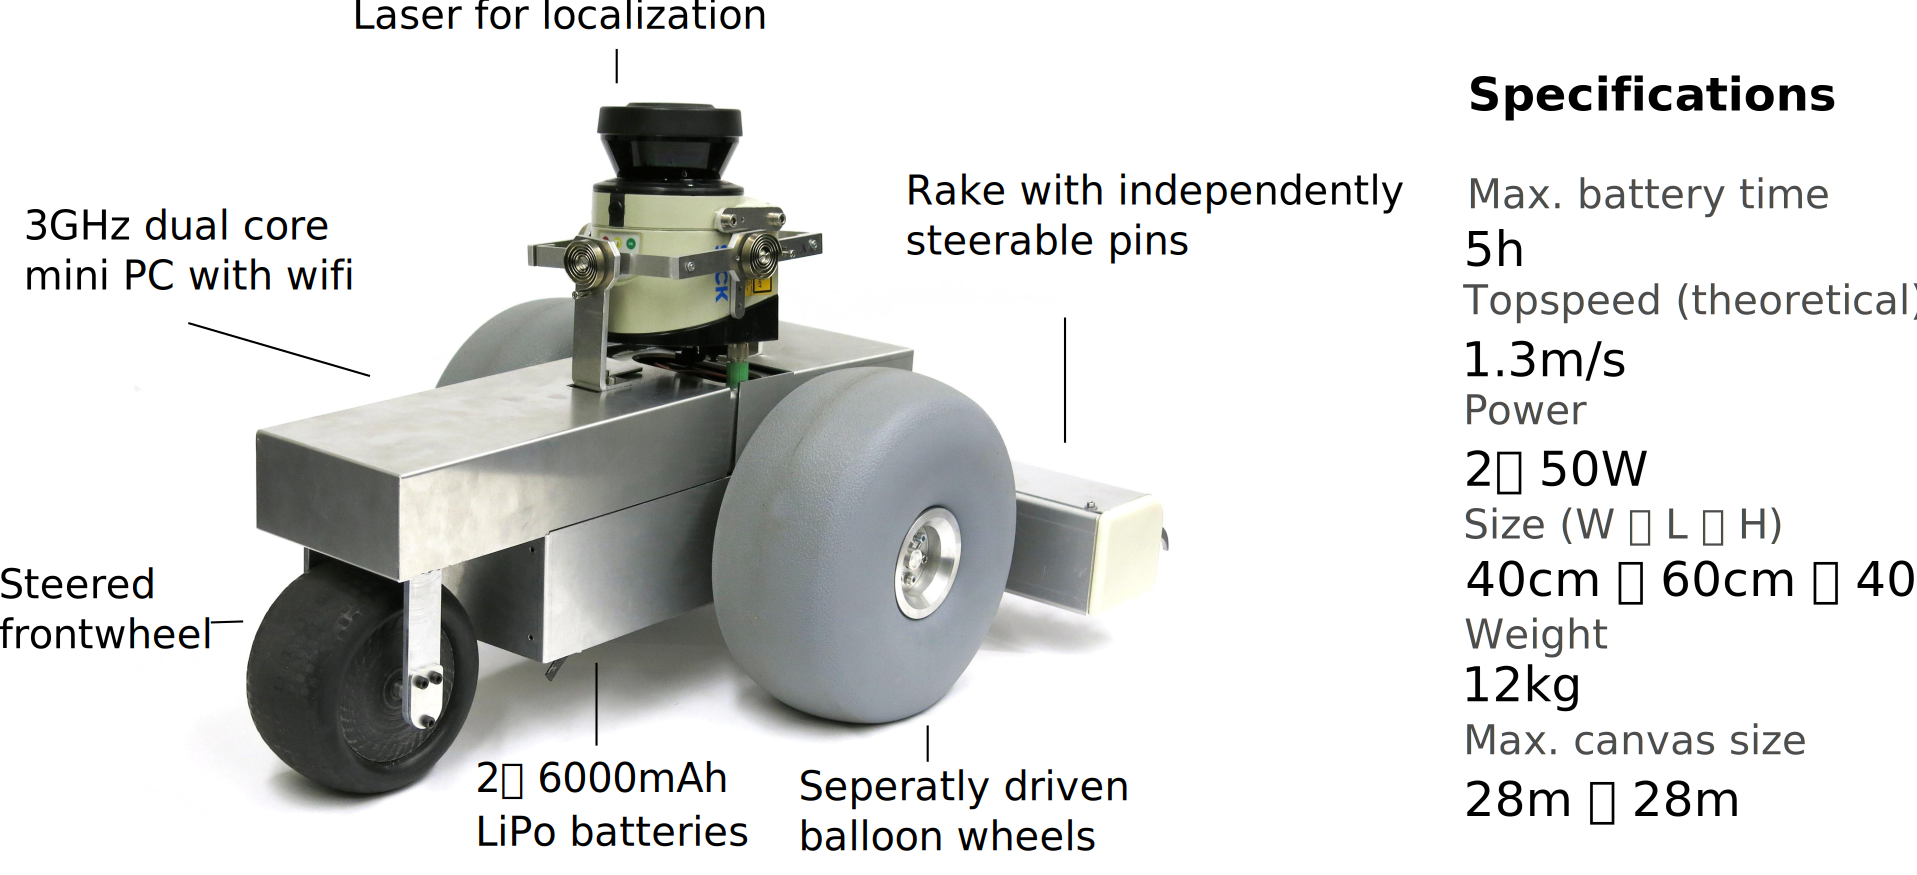
\includegraphics[width=\textwidth]{images/introduction/beachbot_spec.pdf} 
\end{subfigure}
\\
\begin{subfigure}[c]{0.46\textwidth}
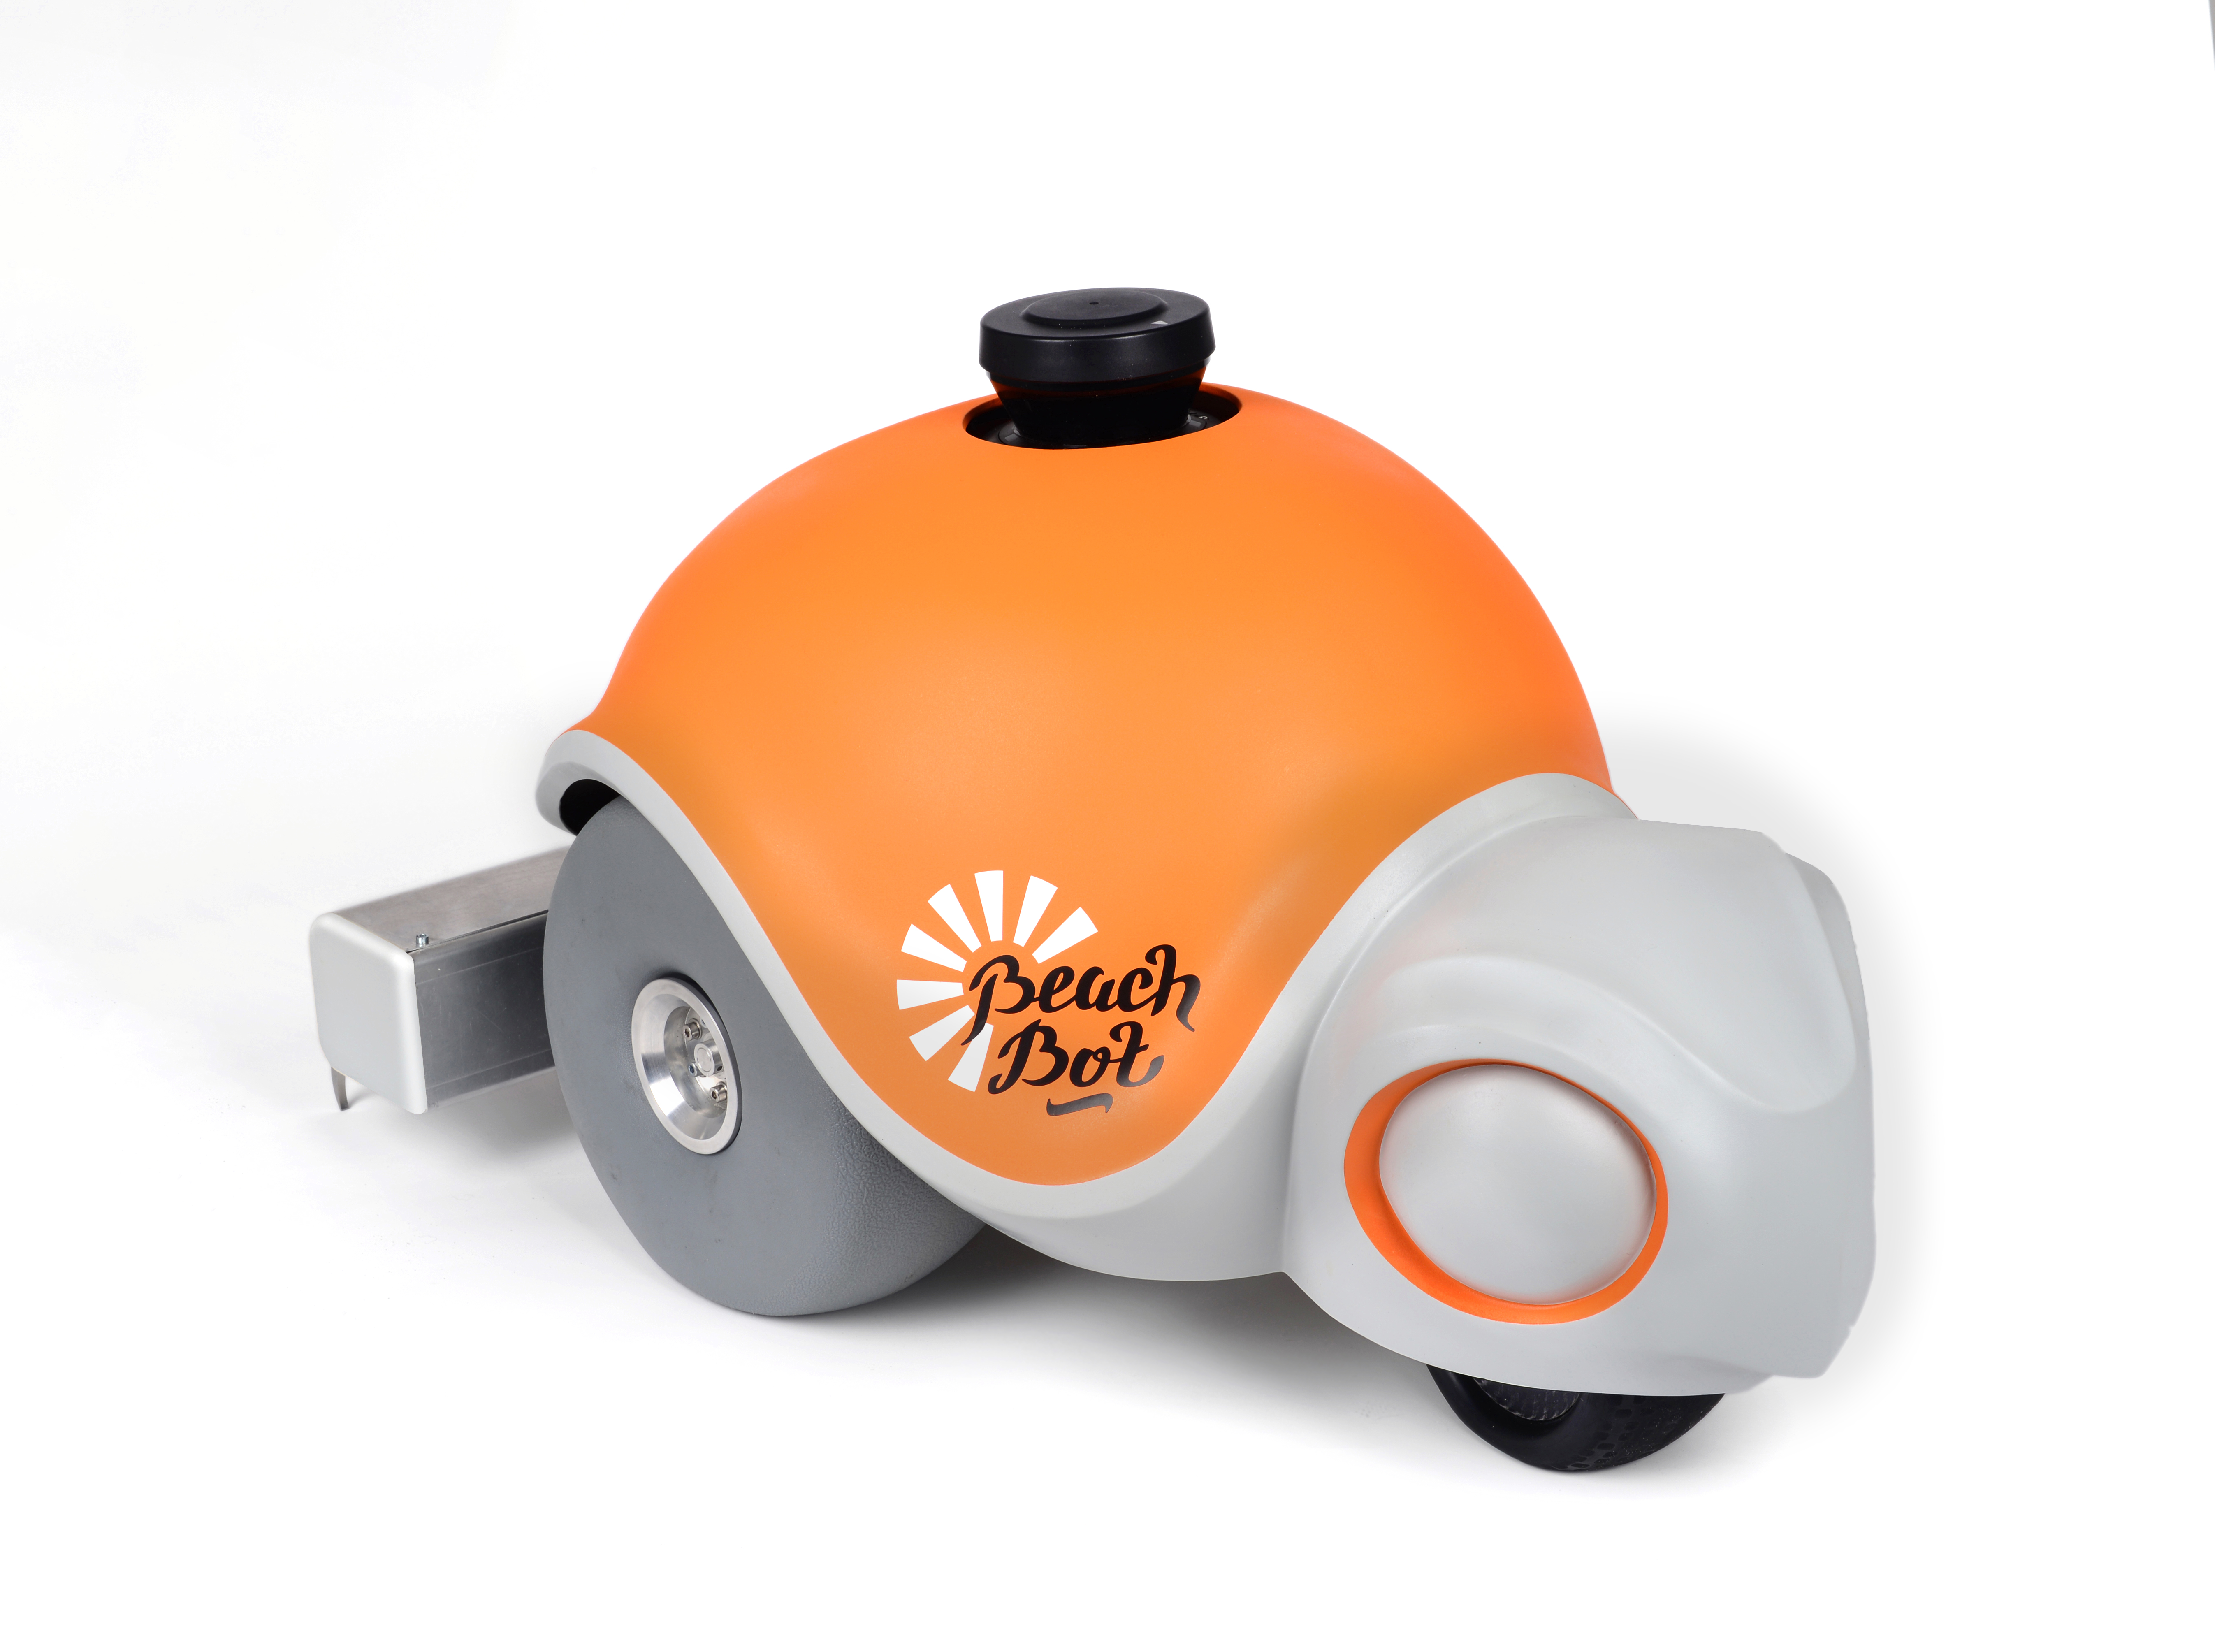
\includegraphics[width=\textwidth]{images/introduction/final_shell.jpg} 
\end{subfigure}
\\
\vspace{2cm}
\begin{subfigure}[c]{0.46\textwidth}
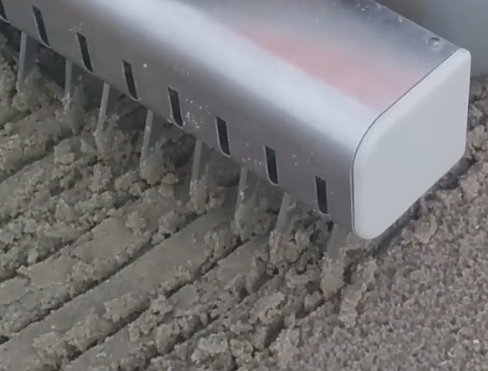
\includegraphics[width=\textwidth]{images/introduction/localization_precision.png} 
\end{subfigure}
~
\begin{subfigure}[c]{0.46\textwidth}
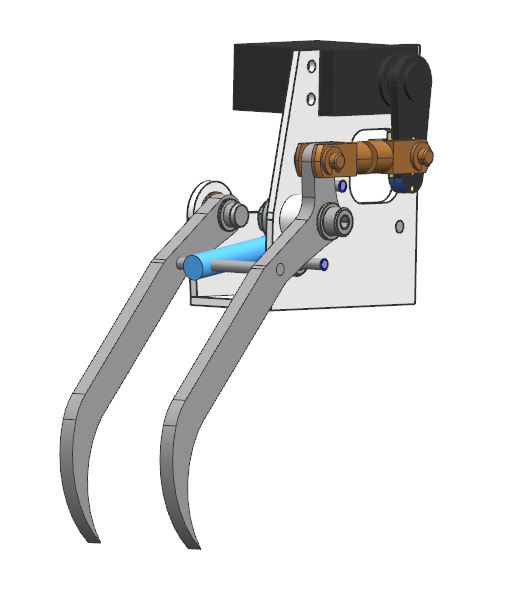
\includegraphics[width=\textwidth]{images/introduction/rake_pins.png}
\end{subfigure}
\caption{Various images of the BeachBot}
\end{figure} 
